\chapter{Performance Optimization}\label{sec:performance} \indexmain{performance}\indexmain{optimization}

The most important point to understand when optimizing for speed is that the expensive task is the search carried out during pattern matching. The effort for rewriting, the dominant theme in graph rewriting (theory) literature, is negligible.

Searching is carried out with a backtracking algorithm following a search plan in a fixed order, 
binding one pattern element after another to a graph element, checking if it fits to the already bound parts.
If it does fit search continues trying to bind the next pattern element (or succeeds building the match object from all the elements bound if the last check succeeds), if it does not fit search continues with the next graph element; if all graph element candidates for this pattern element are exhausted, search backtracks to the previous decision point and continues there with the next element.

Typically, first a graph element is determined with a lookup operation reaching into the graph, binding the element to a graph element of the required type -- the less elements of that type exists, the better -- then neighbouring elements are traversed following the graph structure, until a match of the entire pattern is found.


%%%%%%%%%%%%%%%%%%%%%%%%%%%%%%%%%%%%%%%%%%%%%%%%%%%%%%%%%%%%%%%%%%%%%%%%%%%%%%%%%%%%%%%%%%%%%%%%
\section{Search Plans}

A search plan for the pattern in figure \ref{perf:figpatterntosearch} is:\\
\texttt{lkp(v1:A); out(v1,e1:a); tgt(e1,v2:B); out(v2,e3:b); tgt(e3,v3:C); out(v3,e2:a)}\\
The search operations \texttt{lkp} denotes a node (or edge) lookup in the graph, \texttt{out} follows the outgoing edges of the given source node and \texttt{in} follows the incoming edges ot the given target node, while \texttt{src} fetches the source from the given edge and \texttt{tgt} fetches the target from the given edge.

For some graphs the search plan might work well, but for the graph given in figure \ref{perf:figgraphtosearchin} it is a bad search plan.
Why so can be seen in the search order sketched in figure \ref{perf:figbadsearch}.
Due to the multiple outgoing edges of \texttt{v1} of which only one leads to a match it has to backtrack several times.

This schedule in contrast is a a good one:\\
\texttt{lkp(v3:C); out(v3,e2:a); tgt(e2,v2:B); out(v2,e3:b); in(v2,e1:a); src(e1,v1:A)}\\
corresponding to the search order depicted in figure \ref{perf:figgoodsearch}.

It is crucial for achieving high performance to prevent following graph structures splitting into breadth as given in this example, and especially to avoid lookups on elements which are available in high quantities.

\begin{figure}[p]
  \centering
  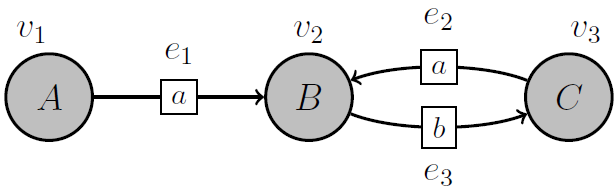
\includegraphics[width=0.7\textwidth]{fig/Pattern}
  \caption{Pattern to search}
  \label{perf:figpatterntosearch}
\end{figure}

\begin{figure}[p]
  \centering
  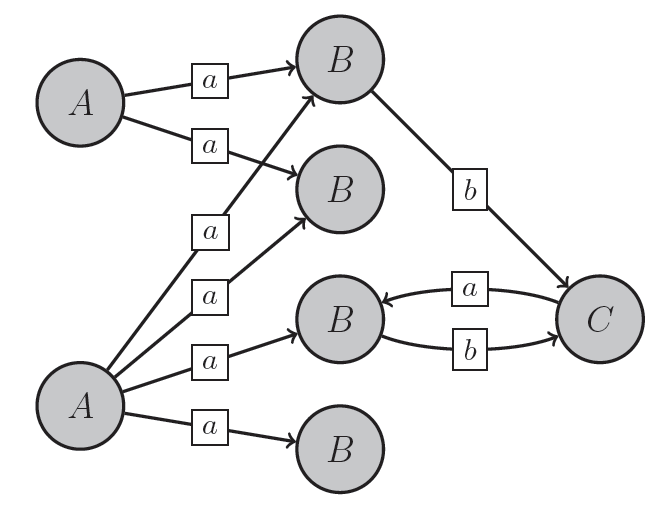
\includegraphics[width=0.7\textwidth]{fig/Graph}
  \caption{Host graph to search in}
  \label{perf:figgraphtosearchin}
\end{figure}

\pagebreak

\begin{figure}[p]
  \centering
  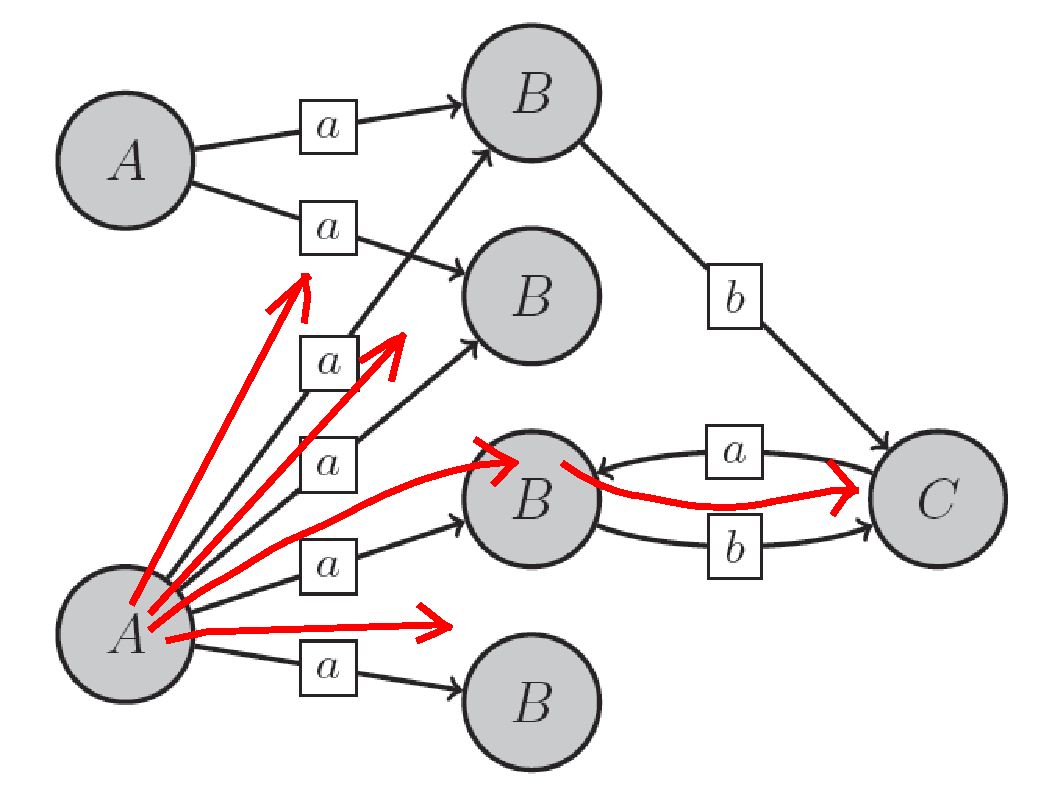
\includegraphics[width=0.7\textwidth]{fig/GraphBad}
  \caption{Bad search order}
  \label{perf:figbadsearch}
\end{figure}

\begin{figure}[p]
  \centering
  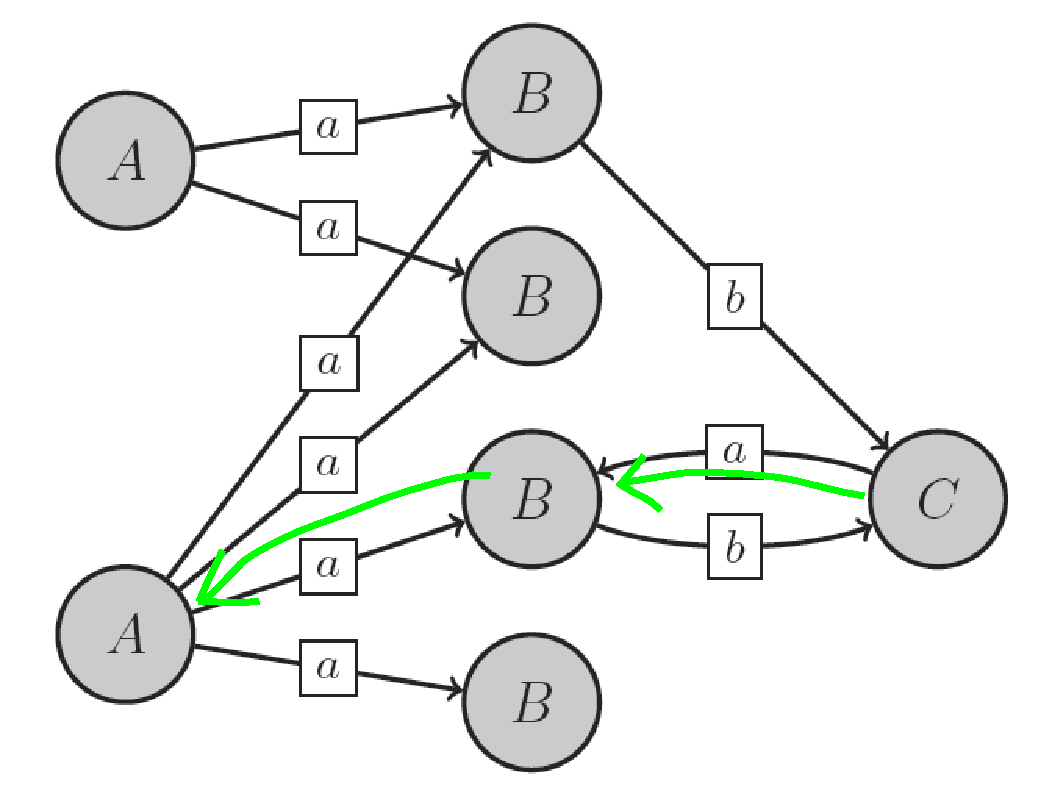
\includegraphics[width=0.7\textwidth]{fig/GraphGood}
  \caption{Good search order}
  \label{perf:figgoodsearch}
\end{figure}


%%%%%%%%%%%%%%%%%%%%%%%%%%%%%%%%%%%%%%%%%%%%%%%%%%%%%%%%%%%%%%%%%%%%%%%%%%%%%%%%%%%%%%%%%%%%%%%%
\section{Find, Don't Search}
Better than searching for elements with certain characteristics, 
traversing each and every node or edge in the graph, 
subjecting it to a test for the characteristic,
is to find them straight ahead without search,
utilizing a data structure that allows to tell the elements that follow the characteristic apart from the ones that do not.
Welcome to indices as known from database parlance.
In \GrG{} we know of four classes of indices:
\begin{enumerate}
	\item Type indices
	\item Neighbourhood indices
	\item Name index
	\item Attribute indices (plus incidence count)
\end{enumerate}

%-----------------------------------------------------------------------------
\subsection{Type Indices}
All the nodes or edges in \GrG{} of a certain type are contained in a list that can be acessed in $O(1)$ and iterated in $O(k)$ with $k$ being the number of elements in that list (the nodes or edges of same type), in contrast to $n$, being the number of nodes or edges in the graph.
The first node or edge in a pattern is typically bound by iterating such a type list.
In case the pattern is disconnected, a lookup is needed per connected component.
In case multiple types have very few members, the search planner may decide to use several lookups even in case of a connected pattern.
(This can be especially the case for reflexive marker edges pointing to the current point of processing/focus of attention in the graph.)

%-----------------------------------------------------------------------------
\subsection{Neighbourhood indices}
All the edges outgoing from a node are contained in a list that can be accessed in $O(1)$ and iterated in $O(k)$ with $k$ being the number of elements in that list (the outgoing edges).
All the edges incoming to a node are contained in a list that can be accessed in $O(1)$ and iterated in $O(k)$ with $k$ being the number of elements in that list (the incoming edges).
So following neighbouring elements, crawling alongside the structure is very cheap in \GrG{ } -- and possible in both directions, following the edges as well as in their opposite direction.

It is cheap in graph databases, too, but absolutely not in relational databases.
To follow a relation, there you have to join two complete tables, building the cartesian product of two tables (materializing only the rows where they agree).
Typically you optimize this with a database index that allows to find the elements of the second table matching your focused element of the first table in $O(log(n))$ -- but for large $n$ or for complex queries this global product is way less efficient than direct local access to exactly the neighbouring elements.
(Furthermore, a table join is conceptionally and notationally much heavier than an edge in a graph pattern).

In case of undirected edges, or arbitrary directed edges in the pattern, both directions are searched,
both lists -- the outgoing list as well as the incoming list -- are crawled.

%-----------------------------------------------------------------------------
\subsection{Consequences}

\subsubsection*{Use types!}
Fine grain types cause a fast lookup of the first pattern element(s).
And they cause quicker pruning of match extensions because of early failing type checks.
Using fine-grain types is easy in GrGen, for multiple inheritance on node and edge types (cf. \ref{nodeandedgetypes}) is supported.
Besides, the more fine grain the graph is typed, the better are the statistics, allowing \GrG{ } to find better search plans (see more for this below).

\subsubsection*{Prefer directed edges}
Non-directed edges in the pattern are searched in both directions, considerably increasing the search space.
Use non-directed edges only if they you really needed them.
For some problems this is the case, you then simply have to pay the price of the increased effort for the symmetry.
But some problems where undirected edges are more natural can be easily encoded with directed ones -- in case of performance problems, refactor and optimize them to employ only directed edges, imposing an arbitrary but deterministic direction on the edges.
Besides, the vstructure statistics are more discriminating in case of directed edges, leading to better search planning results; in case of undirected ones the information from both directions is coalesced.

\subsubsection*{Beware of Disconnected Patterns}
Disconnected patterns cause a combinatorial explosion of the matches, because the overall number of matches equals the cartesian product of the partial matches of the disconnected parts. 

For a single pattern this is normally not specified, and pretty easy to spot.
And if specified, you normally only search for one match of such a pattern, aborting search as soon as found.
But take care of not disconnecting patterns with subpatterns and nested patterns (esp. when factoring out a common part into a subpattern).

Subpatterns are searched top-down (cf. \ref{pushdownmachine}), from the input parameters on.
If the input arguments are disconnected in the pattern containing the subpattern, the containing pattern enumerates the cross product of the matches of the disconnected parts, which is then later on filtered in the subpattern called for the ones which are connected.
This will likely wreak havoc on the search performance.
Even if you don't search for all matches, to compute a single overall match, the calling pattern must enumerate a lot of combinations of its parts that are typically often found because of their simlicity, until the nested pattern finally is able to connect one of the disconnected pairs fed into it.
It might be more efficient to just search from a start parameter a connected end location, and yield the found one out (cf. \ref{sec:localvarorderedevalyield}), or to search from a start parameter all connected end locations, collecting the found ones in a result set; and to check the ones found alongside connectedness in a second step.

The same holds for the nested patterns, just that parameter passing is implicit there, the elements from the containing pattern which are referenced in the nested pattern are passed in automatically as arguments.
The holds especially for the \texttt{alternative} and \texttt{iterated} constructs which are matched with the pushdown machine (cf. \ref{pushdownmachine}), too, but also for the \texttt{negative} and \texttt{independent} constructs which are matched with nested local code embedded into the matcher code of their containing pattern.

Don't shy away from using subpatterns too easily, subpattern \indexed{inlining} is helping here. 
A subpattern is often inlined into the using pattern, causing the pattern to get connected (again); 
additionally removing the pushdown machine overhead.
But you must take into account that the \emph{subpattern inlining} implemented in GrGen is limited to depth one.
If a pattern is disconnected over two or more levels of subpattern usage (which might happen statically with one subpattern using another subpattern, and will for sure dynamically on a subpattern recursion path), it will hit performance.
You may have a look at the output of the \texttt{explain} command (cf. \ref{custom}) to see  if the subpatterns are disconnected; this is typically indicated by multiple lookups in the containing pattern, and the fact that the starting points passed as preset parameters to the nested or subpatterns get connected only there with search commands.

%-----------------------------------------------------------------------------
\subsection{Search planning}
Search planning is only carried out on request!
You must analyze the graph and then re-generate the matchers at runtime,
with \texttt{custom graph analyze} and \texttt{custom actions gen\_searchplans} (issued on the command line or to the \texttt{Custom}methods of the graph and the actions objects);
you may have a look at the effects of replanning with the \texttt{custom actions explain <actionname>} command.
See subsection \ref{custom} for more on this.

The initial static search plans start with a lookup of an arbitrary edge, and then arbitrarily follow graph structure.
Interestingly, in many cases this still works quite well because of the quick pruning of the type checks in a well-typed graph.
In addition, often the rules work from some parameter nodes onwards, which are typically well suited start points for search.

You can inspect the current search plan employed wit the explain command.
Use it before search planning to inspect the statically generated search plans.
Use it afterwards to inspect how the elements are matched now.

dynamic analyze better than mostly random static ones, sometimes you may be better by assigning priorities
You may improve the static schedules by explicitly giving search priorities.

Again: Use types!
The more fine grain a graph is typed, the better are the statistics regarding the splitting factors (V-Structures) and the number of elements of a certain type, yielding better search plans evading splitting structures and employing least-cost lookups, pruning non-matches earlier in the search.

%-----------------------------------------------------------------------------
\subsection{Name Index}
A named graph is a graph where each element bears a unique name and can be looked up quickly by that name.
So basically it works as a graph with an integrated key-value store from a string to graph elements; and from graph elements to their string.
It is implemented with two hash maps, one from the name to the elements, and the other from the elements to the name.
Lookup is carried out in $O(1)$.
Maintaining the index on graph insertions and removals is carried out in $O(1)$, too.
If you are working with the Shell, this is the only kind of graph you'll be working with.
At API level you may opt for the non-named graph that are considerably cheaper regarding memory usage -- a named graph requires not much less than about twice the amount of memory of a plain graph.
But please note that the export and import capabilities require uniquely named elements and thus only work with named graphs.
If given a plain graph the exporters just creates a named graph, and a graph is always read in as a named graph.
So non-named graphs are only of interest if you don't need to persist them into a serialization format.
Futhermore, only the named graph supports attribute indices or incidence count indices, 
as the names are needed for ordering attributes with the same value or nodes with same incidence count.

%-----------------------------------------------------------------------------
\subsection{Attribute Indices}
The type and neighbourhood indices are built into each and every \GrG{} graph, wired into a system of ringlists (cf. \ref{}).
You always benefit from them during matching (most if you are using statistics-based search planning), but you must always pay their price:
The memory consumption of a \GrG{} node without attributes is 32 bytes using a 32bit CLR (5 pointers a 4 bytes, a 4 bytes flags field/bitvector plus 8 bytes .NET object overhead), it is 60 bytes for a 64bit CLR (5 pointers a 8 bytes, a 4bytes flags field, plus 16 bytes .NET object overhead).
The memory consumption of a \GrG{} edge without attributes is 48 bytes using a 32bit CLR (9 pointers a 4 bytes, a 4 bytes flags field/bitvector plus 8 bytes .NET object overhead), it is 92 bytes for a 64bit CLR (9 pointers a 8 bytes, a 4 bytes flags field, plus 16 bytes .NET object overhead).
Attributes only increase this by the .NET-memory-footprint of their underlying objects.
The runtime price of those indices during graph manipulation is low, adding a graph element is done in $O(1)$, removing a graph element is done in $O(1)$, too. 
(Furthermore, those indices allow to optimize loops by starting matching where the previous iteration left of (search state space stepping)).
We consider this the best you can get for the task of efficient pattern matching on typed, attributed multigraphs -- those indices are simply worth their price in the general case (you can only improve on this by exploiting the specifics of a less general graph model or by restricting yourself to less general pattern matching).

In addition to those built-in indices, you may declare attribute indices or special-purpose incidence count indices.
An attribute index allows to do a lookup based on an attributes value, or a range of attribute values.
In contrast to the default behaviour of carrying out a lookup on a type, visiting all $n$ elements of the type, filtering them down to the elements of interest (within range) with an attribute condition.
If this means you have to inspect a lot of values while searching only for a few ones, you should use an attribute index and benefit from its massively improved selectiveness for the lookup.
It requires only $O(log(n))$ to search for the first element, and $O(k)$ for the $k$ elements within the bounds specified.
It is implemented with a balanced binary search tree (an AA-tree\cite{} to be exact) that requires three pointers plus one 4 byte integer per element contained in the index (two pointers to the left and right tree nodes, and one to the graph element as value), which is really cheap.
But it must be maintained on graph changes, which is less cheap.
On each and every graph element insertion and removal, but esp. attribute assignment, the index needs to be updated, which is an $O(log(n))$ operation.
That's only logarithmic, but clearly worse than the default $O(1)$ behaviour of \GrG{}, so if you do a lot of graph manipulations and only few lookups based on it, an index may in fact degrade performance.

\subsubsection*{Incidence Count Indices}
If you need to find out often the amount of incident edges, have an algorithm that works best when applied to the most heavily connected nodes first.


%%%%%%%%%%%%%%%%%%%%%%%%%%%%%%%%%%%%%%%%%%%%%%%%%%%%%%%%%%%%%%%%%%%%%%%%%%%%%%%%%%%%%%%%%%%%%%%%
\section{Location passing and memorization}
Often in a transformation you know the location you want to process from a previous step.
In this case, store these locations in variables of node (or edge) type, and hand them in as parameters to the rules and return them out from the rules.

Commonly, this is just the right way of handling this, 
as you must continue processing the very spot you just processed with the previous rule(s).
Sometimes you don't need to, but gain higher performance when you do so.
Optimize this way then (use rooted pattern matching, with roots defined by previous rules), it's cheap and easy.
A different way of parameter passing is adding reflexive edges to the graph to mark the spot of processing.
This is normally working well, but the parameter passing is typically easier and does not "`pollute"' the graph with processing information.
It also works in case of an unbounded number of processing locations, that cannot be handled with a statically bound number of variables.

But in case of a statically not known number of locations as they appear e.g. in wavefront algorithm, you may store the locations in storages (cf. chapter \ref{cha:container}), i.e. collection valued variables (which are iterated over in the sequences or passed to the rules as \texttt{ref} parameters).
Search will then start from these parameters, instead of a looking up a value in the graph by type (unless search planning taking the statistics about the graph into account comes to the conclusion  that a lookup on a very seldom type is still the better approach).

A sophisticated way of remembering facts about non-local properties is to computed them with data flow analyses (see section \ref{subsub:flow}) and store them as attributes in the graph elements.
This allows to replace searching for distant values, or global properties like reachability, by checking a local property, at the price of re-running an analysis every time the graph changes in an important way.

Speaking in database parlance, with storages you can build indices into the graph, indices which are more selective than the automatically built indices by graph element type; but in contrast to the automatically built ones, you must maintain them by hand.

The approach of remembering state instead of searching when needed has a clear caveat: the code becomes less readable and more brittle. As in normal programming, you must balance performance optimizations against maintainability.

In contrast to the 3 previous classes of indices that are maintained by the \GrG{} graph, you must maintain them on chnages by hand.


%%%%%%%%%%%%%%%%%%%%%%%%%%%%%%%%%%%%%%%%%%%%%%%%%%%%%%%%%%%%%%%%%%%%%%%%%%%%%%%%%%%%%%%%%%%%%%%%
\section{Profile and Parallelize}

A basic and often fully sufficient means of profiling is built-in into GrShell:
After each sequence execution the time required to carry it out is printed.

Sometimes you need further information about what's going on.
Profile. 
Tells you about search steps carried out.

Parallelize.
Use the annotation to parallelize the first loop of a pattern.
The normal pattern matchers of \GrG{ } are highly efficient, in the common case a parallelization will lead to a performance degradation because of the threading and locking overhead.
Use this only selectively. Profile to find out where it may be worth it. Take a look at the execution times to see if it really is better.

%%%%%%%%%%%%%%%%%%%%%%%%%%%%%%%%%%%%%%%%%%%%%%%%%%%%%%%%%%%%%%%%%%%%%%%%%%%%%%%%%%%%%%%%%%%%%%%%
\section{Compilation and static knowledge}

\subsubsection*{Use saved graph analyzation data}
Save graph analyze information after analyzing a characteristic graph.
Use it by generating static matchers adapted to this characteristic graph.
It's very seldom you really need dynamic information, and most often it's not worth it, as graph analyzation and matcher generation are costly.

\subsubsection*{Use Compiled Sequences}
The compiled sequences given in the rules file are executed a good deal faster than the interpreted sequences given in the shell.
So if you need speed, replace interpreted sequences by compiled ones.
The price you pay is a loss of debuggability, a compiled sequence can only be executed as one big step.

\subsubsection*{Use Pre-Compiled Code}
For shortly-running tasks the JIT-compiling overhead dominates the runtimes.
TODO.


%%%%%%%%%%%%%%%%%%%%%%%%%%%%%%%%%%%%%%%%%%%%%%%%%%%%%%%%%%%%%%%%%%%%%%%%%%%%%%%%%%%%%%%%%%%%%%%%
\section{Miscellaneous Things}

\subsubsection*{Visited flags}
Visited flags are the most efficient way of marking elements, if a large number of the elements gets marked.
Otherwise they are inefficient, cause a lot of elements need to be iterated, just to filter the visited ones out.
Storages which give quick access to their contained elements are better then.
Or even reflexive marker edges of a special type in the graph, search planning favors them.

\subsubsection*{Loops}
The loops are very efficient due to search state space stepping, continuing where the last iteration left of.
Still, you should prefer all-bracketing (cf. \ref{sec:ruleapplication}) over iteration for rule application.
This holds for case that you really want to execute a rule on all matches that are available at a point in time, and not on other matches that were not available originally at the first rule application.
Utilizing a loop in that situation would simply yield semantically different results.
But even if this is not the case, you should use an all-bracketed rule if it works.
Please not that this is only possible if the parts of the matches which are to be modified, e.g. retyped, are disjoint.

